\documentclass{./../div_teaching_slides}

\begin{document}
\title{ECON 340 \\ Economic Research Methods}
\author{Div Bhagia}
\date{Lecture 18 \\ Omitted Variable Bias, Multiple Regression Model}

%%%%%%%%%%%% 
\begin{frame}[noframenumbering, plain]
\maketitle
\end{frame}

%%%%%%%%%%%% 
\begin{frame}{Test Scores and Class Size}
\vspace{-0.5em}
\centering
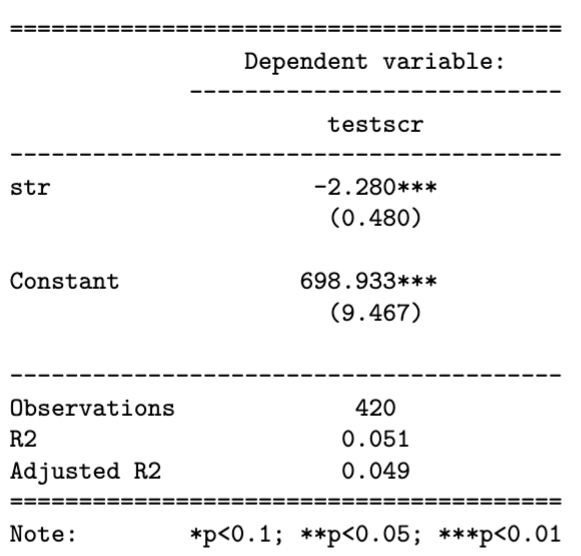
\includegraphics[scale=0.375]{reg_output_stargazer.png}
\end{frame}

%%%%%%%%%%%%%%%%%%%%
\begin{frame}{Omitted Variable Bias}
\begin{witemize}
  \item School districts with lower student–teacher ratios tend to have higher test scores
  \item However, students from districts with small classes may have other advantages that help them perform well
  \item Omitted factors (e.g. student characteristics) can make the OLS estimator biased
  \item Today's lecture: \textit{omitted variable bias} and \textit{multiple regression}, a method that can eliminate this bias
\end{witemize}
\end{frame}

%%%%%%%%%%%%%%%%%%%%
\begin{frame}{Omitted Variable Bias}
Consider the following linear regression model:
$$ Y = \beta_0 + \beta_1 X + u  $$
\vspace{0.25em}

Omitted variable bias occurs when \underline{both} conditions are true: \\  \vspace{0.25em}
\begin{witemize}
  \item[(1)] The omitted variable is correlated with $X$
  \item[(2)] The omitted variable $\rightarrow$ Y
\end{witemize}
\end{frame}


%%%%%%%%%%%%
\begin{frame}{Omitted Variable Bias}
In our example:
$$ Test Score = \beta_0 + \beta_1 \cdot STR + u $$

\textit{Which of these omitted factors will lead to bias?}  \\ \vspace{0.25em}
\begin{witemize}
  \item[(a)] percentage of English learners
  \item[(b)] time of day when tests were conducted
  \item[(c)] parking lot space per pupil
  \item[(d)] computers per student
\end{witemize}

\end{frame}

%%%%%%%%%%%%
\begin{frame}{Omitted Variable Bias}
$$ Y = \beta_0 + \beta_1 X + u  $$
\begin{witemize}
  \item Remember $u$ represents all factors, other than $X$, that are determinants of $Y$.
  \item Omitted Variable Bias means that the exogeneity assumption $E(u|X)=0$ doesn't hold.
  \item If $E(u|X)\neq 0$, OLS estimator is biased.
\end{witemize}
\end{frame}

%%%%%%%%%%%%
\begin{frame}{Omitted Variable Bias}
When $E(u|X)\neq 0$,
$$ \hat{\beta}_1 = \beta_1 +  \frac{Cov(X,u)}{Var(X)} $$

\vspace{1em}
Direction and strength of bias depends on the correlation between $u$ and $X$. \\ \vspace{0.5em} %\pause
%We expect \textit{student-teacher ratio} to be negatively correlated with \textit{computers per student}, i.e. $Cov(X,u)<0$, in which case our coefficient $\hat{\beta_1}<\beta_1$. In other words, $\hat{\beta_1}$ is more negative than $\beta_1$. \\~\\
%Note that here \textit{computers per student} enters $u$ positively. 
\end{frame}

%%%%%%%%%%%%
\begin{frame}{Omitted Variable Bias}
In our example:
$$ Test Score = \beta_0 + \beta_1 \cdot STR + u $$

\textit{What should be the direction of bias due to the following omitted variables?}  \\ \vspace{0.25em}
\begin{witemize}
  \item[(a)] percentage of English learners
  \item[(b)] computers per student
\end{witemize}
\end{frame}

%%%%%%%%%%%%
\begin{frame}{Multiple Regression Model}
$$ Y = \beta_0 + \beta_1 X_{1} + \beta_2 X_{2} + u  $$ 
\begin{witemize}
  \item Again can be used for both purposes, causal inference and prediction
  \item As before we need the data to come from a random sample and no large outliers, but now in addition we also need that $X_1$ and $X_2$ are not perfectly multi collinear. 
  \item Moreover, we can modify the mean independence to:
  $$ E(u | X_1, X_2)=0 $$
\end{witemize}
\end{frame}

%%%%%%%%%%%%
\begin{frame}{Multiple Regression Model}
$$ Y = \beta_0 + \beta_1 X_{1} + \beta_2 X_{2} + u  $$ 
\begin{witemize}
  \item Assumptions: (1) random sample, (2) no large outliers, (3) no perfect multicollinearity, (4) $E(u | X_1, X_2)=0$
  \item Under these assumptions, $\beta_1$ captures the causal effect of $X_1$ keeping $X_2$ constant, and $\beta_2$ captures the causal effect of $X_2$ keeping $X_1$ constant. 
\end{witemize}
\end{frame}

%%%%%%%%%%%%
\begin{frame}{Control Variables}
\begin{witemize}
  \item While there are cases where we might want to evaluate the effect of both the variables, it is hard to find exogenous variables 
  \item A really good use of the multiple regression model is to instead \textit{control} for omitted variable $W$ while trying to estimate the causal effect of $X$
  $$ Y = \beta_0 + \beta_1 X + \beta_2 W + u  $$ 
\end{witemize}
\end{frame}

%%%%%%%%%%%%
\begin{frame}{Control Variables}
  $$ Y = \beta_0 + \beta_1 X + \beta_2 W + u  $$ 
  \begin{witemize}
  \item So instead of assumption (4), we can assume \textit{conditional mean independence}  $$ E(u|X,W) = E(u|W) $$
  \item The idea is that once you control for the $W$, $X$ becomes independent of $u$
  \item Under this modified assumption, we can interpret $\beta_1$ as the causal effect of $X$ while \textit{controlling} for $W$ 
\end{witemize}
\end{frame}

%%%%%%%%%%%%
\begin{frame}{In Summary}
\vspace{-1em}
$$ Test Score = \beta_0 + \beta_1 \cdot STR + \beta_2 \cdot comp\_stu + u $$ \vspace{-0.5em}
\begin{witemize}
  \item Under assumption: 
$$ E(u | STR,comp\_stu)=0   $$
$\beta_1$ causal impact of $STR$, and $\beta_2$ causal impact of $comp\_stu$
\item Under conditional independence: 
$$ E(u | STR, comp\_stu)= E(u |comp\_stu)   $$
$\beta_1$ causal impact of $STR$, and $\beta_2$ could still be biased
\end{witemize}
\end{frame}


%%%%%%%%%%%% 
\begin{frame}{Test Scores and Class Size}
\vspace{-0.5em}
\centering
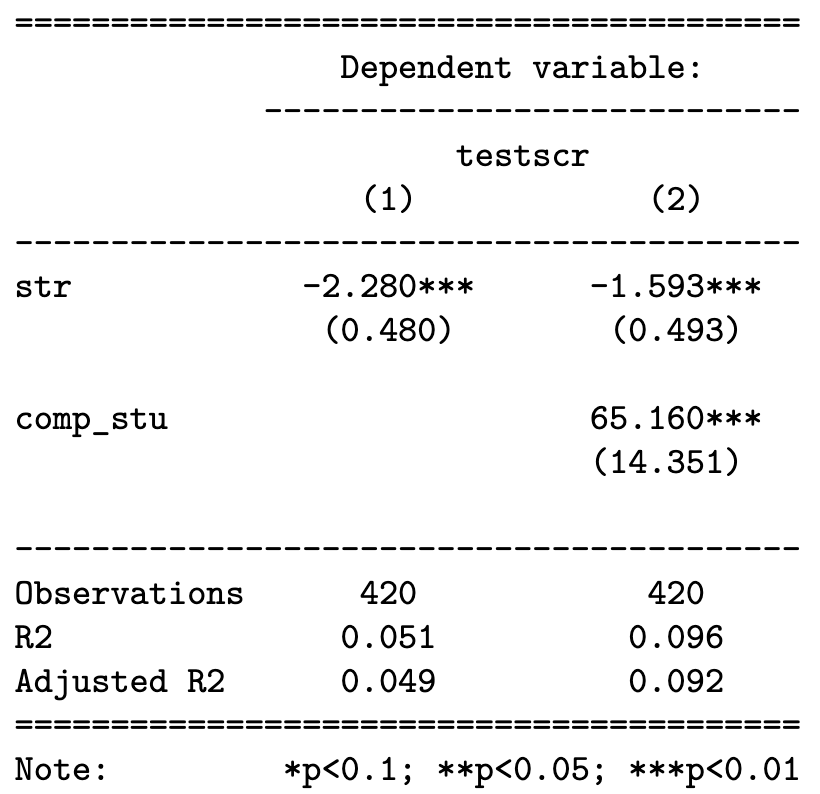
\includegraphics[scale=0.3]{reg_output_stargazer2.png}
\end{frame}

%%%%%%%%%%%% 
\begin{frame}{Goodness of Fit: The $R^2$}
\begin{witemize}
\item[]   \textit{Total Sum of Squares:} $TSS = \sum_{i=1}^n (Y_i-\bar{Y})^2 $
\item[]  \textit{Explained Sum of Squares:} $  ESS = \sum_{i=1}^n (\hat{Y}_i-\bar{Y})^2 $
\item[]   \textit{Residual Sum of Squares:} $  RSS = \sum_{i=1}^n (Y_i-\hat{Y}_i)^2 =\sum_{i=1}^n \hat{u}_i^2$ \\~\\
\end{witemize}
$$ TSS = ESS + RSS $$ \\~\\
A measure of goodness of fit: 
$$ R^2 = \frac{ESS}{TSS} = 1-\frac{RSS}{TSS} $$
\end{frame}

%%%%%%%%%%%%
\begin{frame}{Adjusted $R^2$}
$R^2$ never decreases when an explanatory variable is added \\~\\
An alternative measure called Adjusted $R^2$ 
$$ Adjusted R^2 = 1-\frac{RSS/(n-k-1)}{TSS/(n-1)} $$ 
where $k$ is the number of variables. \\~\\
$Adjusted R^2$ only rises if RSS declines by a larger percentage than the degrees
of freedom.
\end{frame}

\end{document}